%SUBSECTION - control
\subsubsection{Optimal control parameters determination}
As the controller in use is a discrete PID, the first step is to find the optimal parameters.
For the first set of simulations, the aim is to find the values for the PID gains. As purpose of the car is to explore hazardous areas, the parameter $K_d$ will be set as 0 due to the noise. \\
\begin{figure}[!h]
\centering
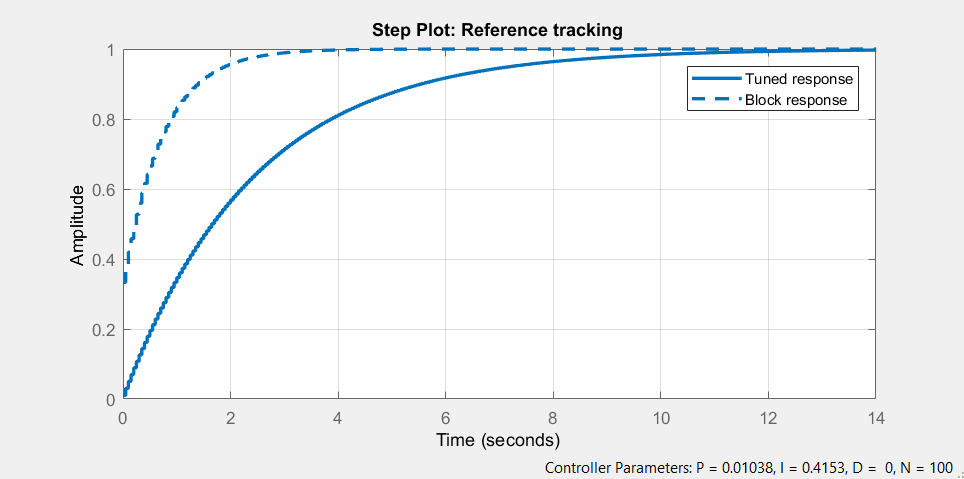
\includegraphics[width=0.8\textwidth]{./img/pidtuned.png}
\caption {\label{fig:pid1-tuned}Automatic matlab tune}
\end{figure}
Resorting the matlab functionality to automatically tune the PID gains for the system, the outcome is the present in the figure \ref{fig:pid1-tuned}. It is possible to see that the velocity of the car reaches the reference value in approximately 11 seconds which is too long. The aim is for the car to get to the speed reference as fast as possible, so, in order for that to happen, new values of $K_p$ and $K_i$ have to be found in simulations.
For the first simulation, $K_p = 1$, $K_i = 1$, Linear speed = 1 m/s, $\theta = 0~\si{rad}$:
\begin{figure}[!h]
\centering
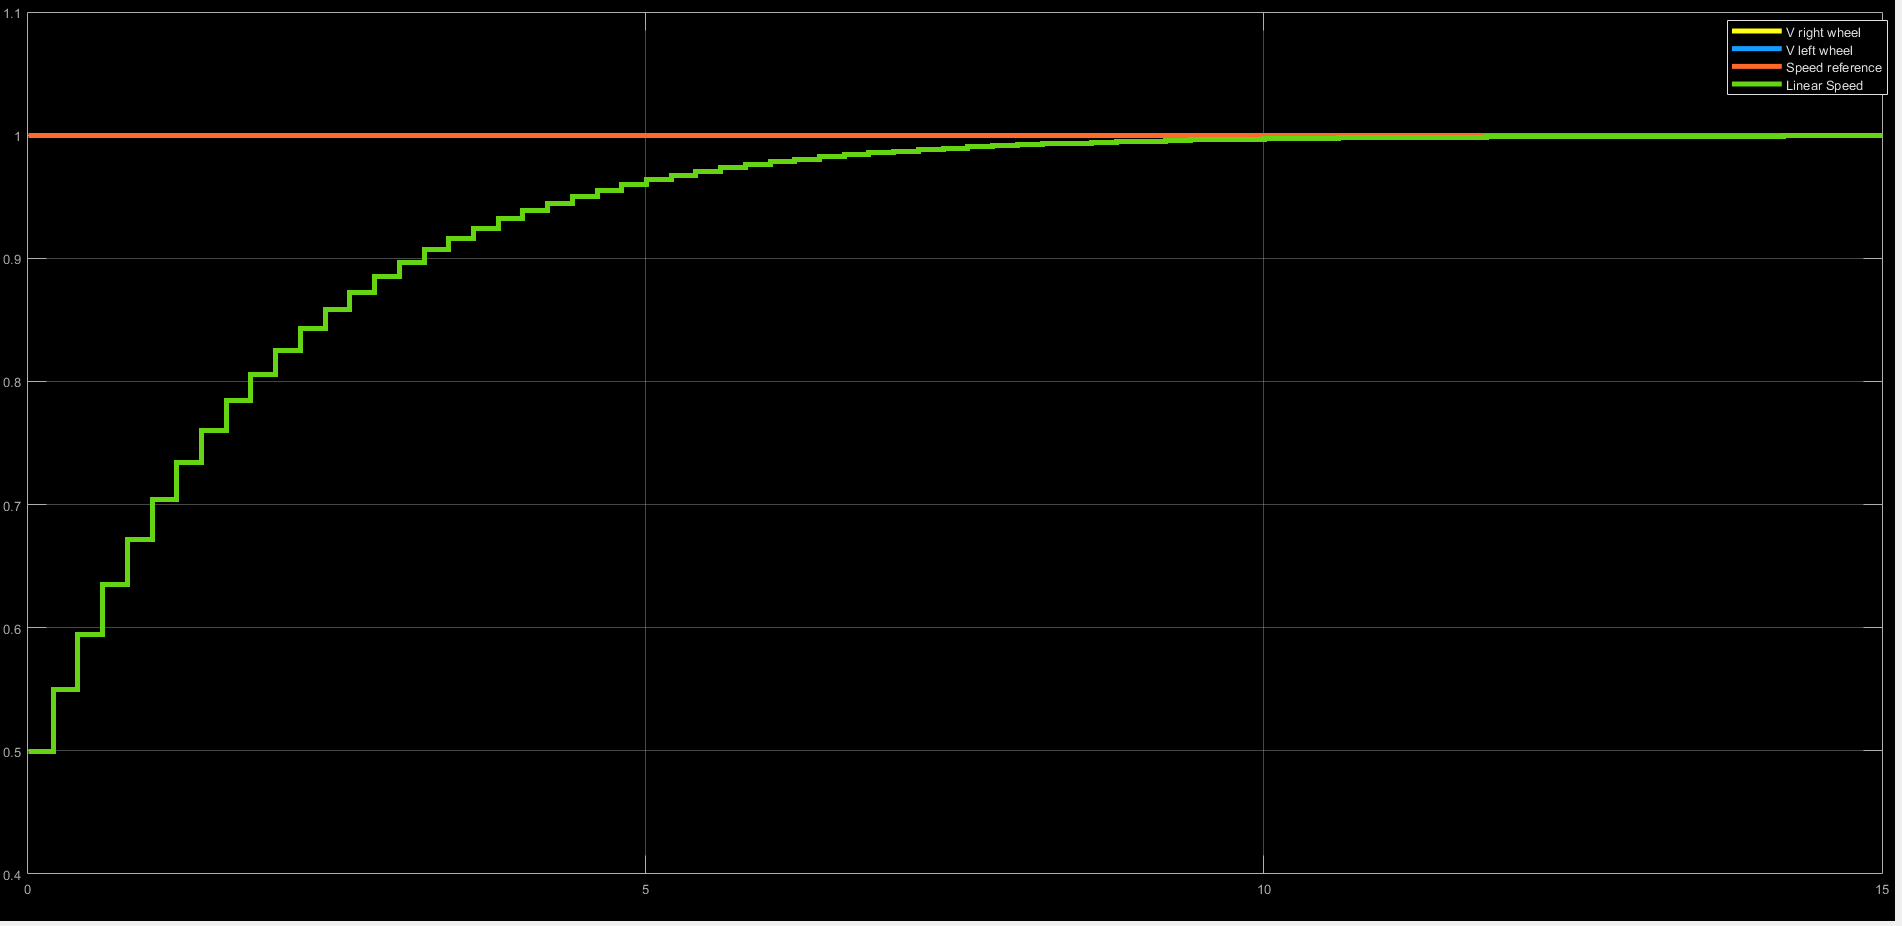
\includegraphics[width=0.8\textwidth]{./img/pid11.png}
\caption {\label{fig:pid1-p1i1}$K_p=1$, $K_i=1$}
\end{figure}
With the figure \ref{fig:pid1-p1i1}, it is possible to see that the initial value of the velocity of the car is 0.5 m/s and it take about 7 seconds to reach steady state. 0.5m/s as an initial value for the linear velocity is a considerably high value and can cause the car to slide, therefore, the $K_p$ value needs to get lower, for the initial value to get lower as well.
%\newpage
In the next simulation \ref{fig:pid1-p05i1}, $K_p$ will be set as 0.5 and $K_i$ as 1.
\begin{figure}[!h]
\centering
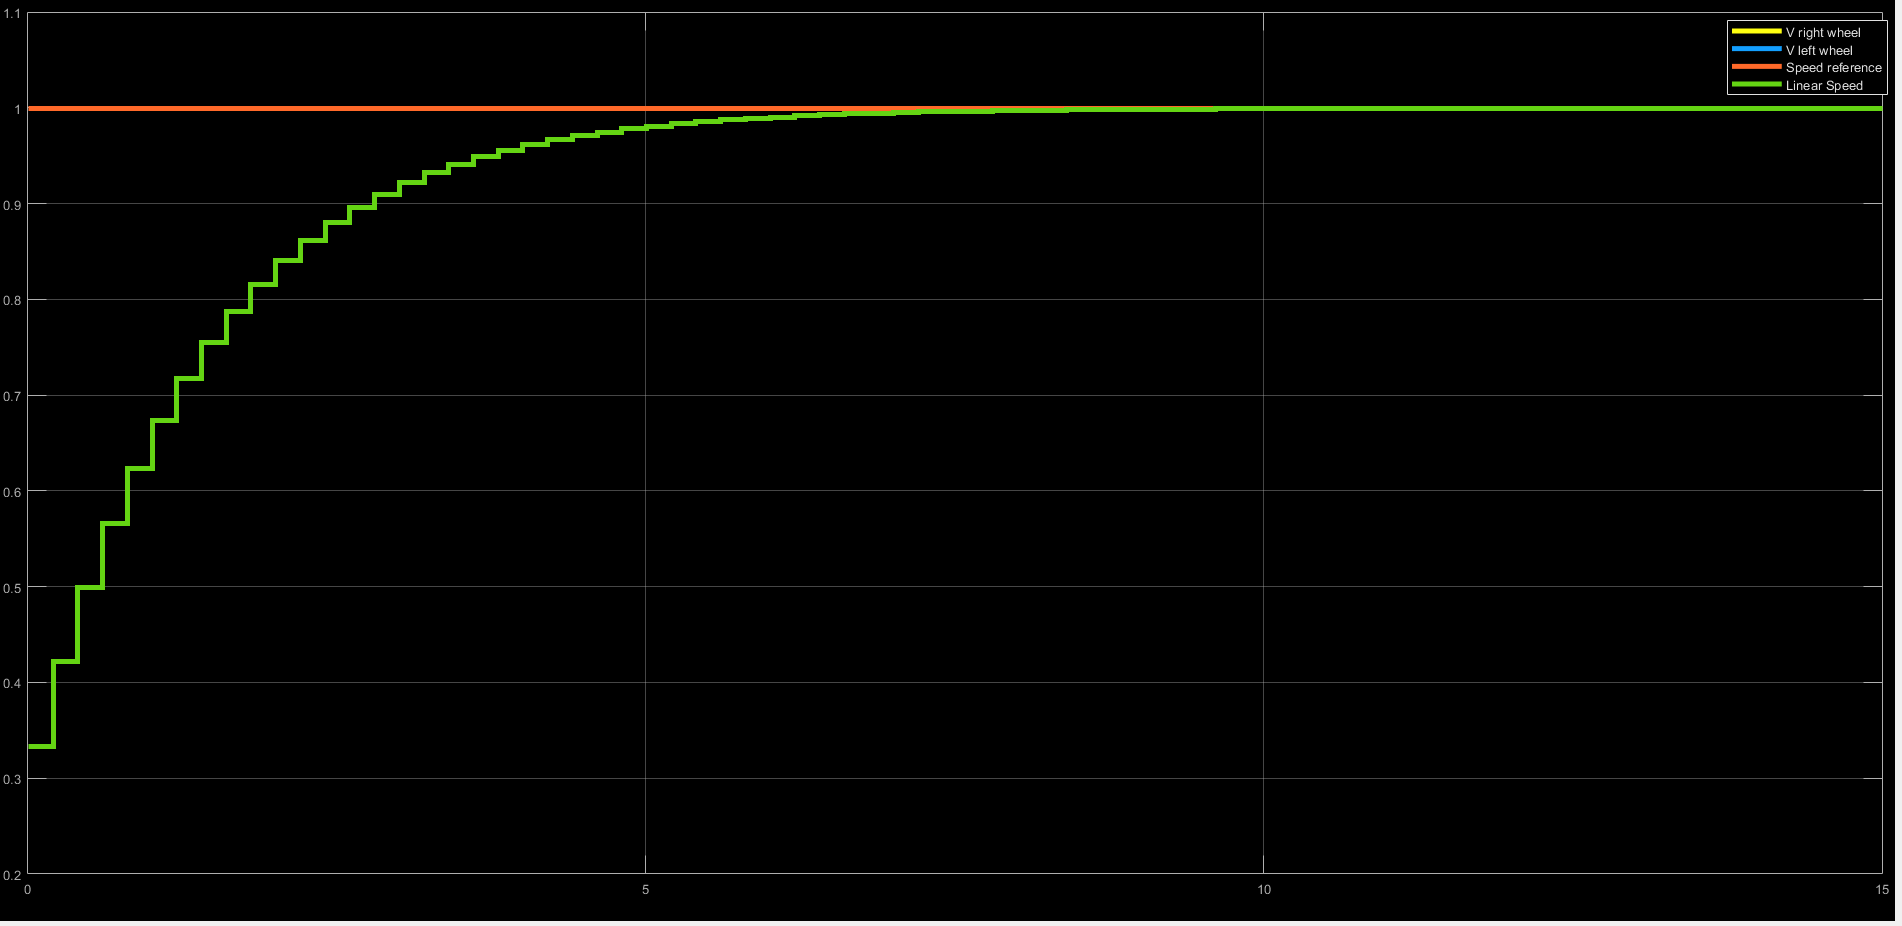
\includegraphics[width=0.8\textwidth]{./img/pid051.png}
\caption {\label{fig:pid1-p05i1}$K_p=0.5$, $K_i=1$}
\end{figure}
Changing the value of $K_p$ to half of the initial value, it is possible to see that the initial linear speed is now 0.3 m/s, making it harder for the car to slide. It takes nearly 6 seconds for the car to reach steady state, thus the $K_i$ value must be increased.
%\newpage
In the next simulation \ref{pid1 - p05i2}, $K_p$ will be set as 0.5 and $K_i$ as 2.
\begin{figure}[!h]
\centering
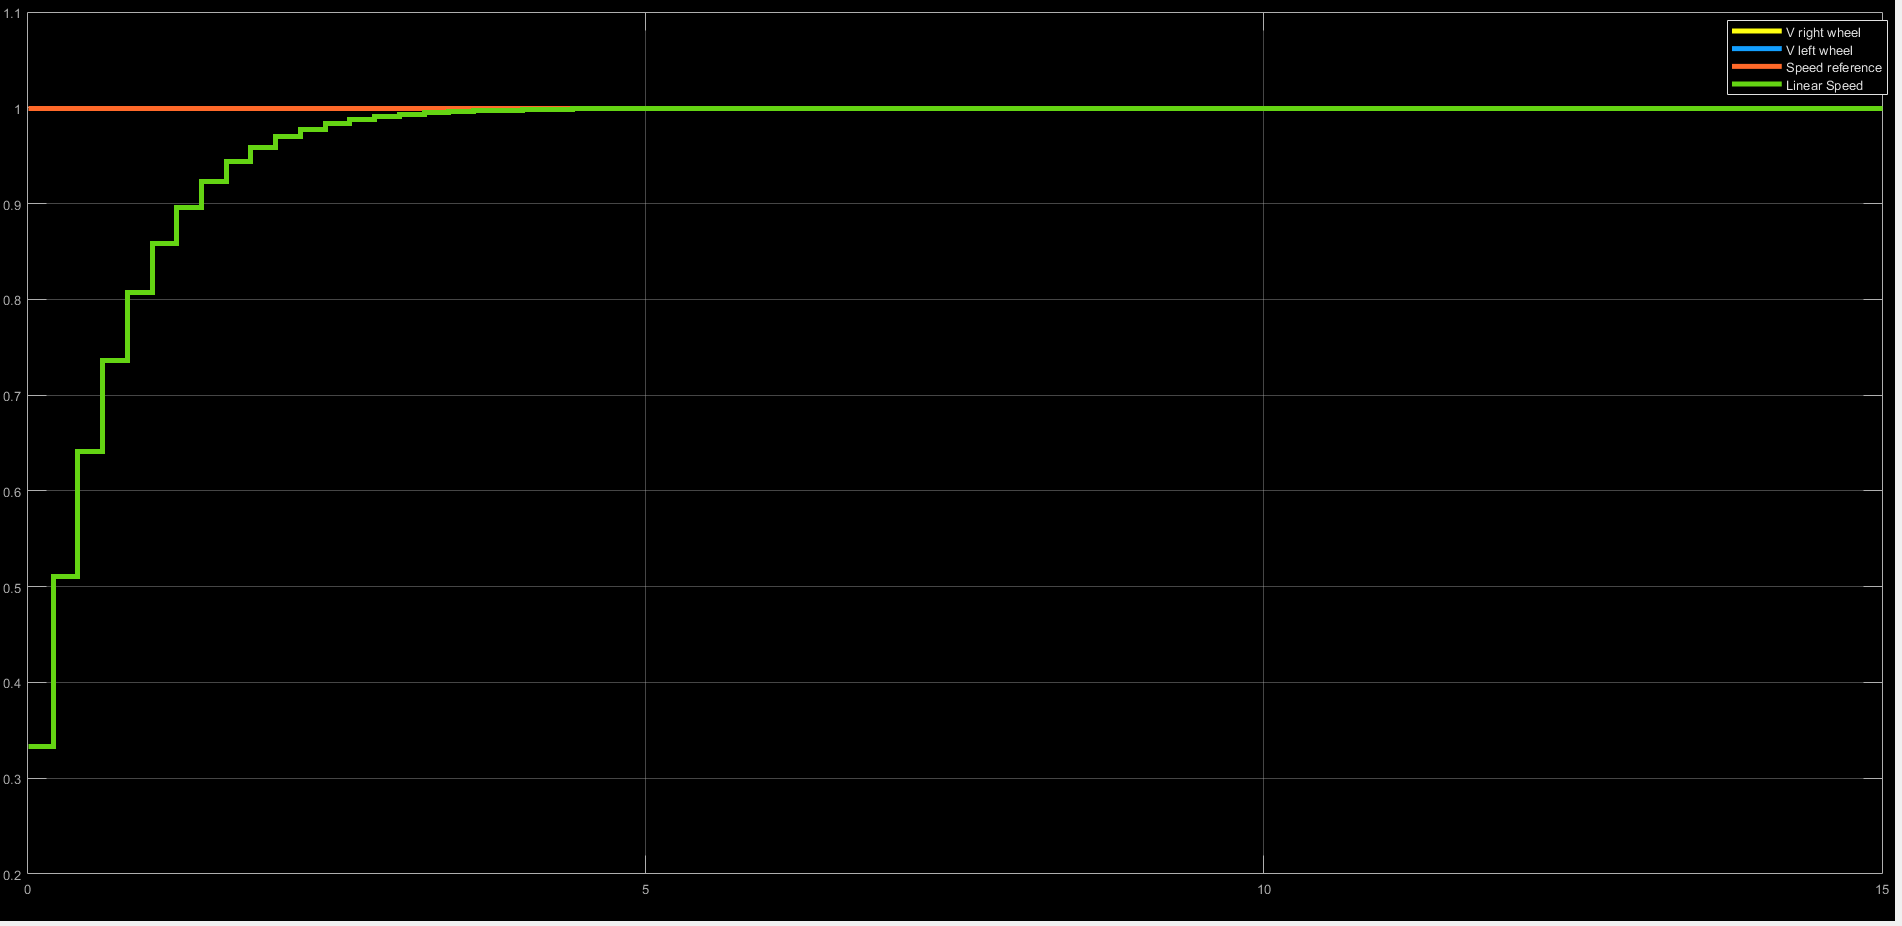
\includegraphics[width=0.8\textwidth]{./img/pid052.png}
\caption {\label{fig:pid1 - p05i2}$K_p=0.5$, $K_i=2$}
\end{figure}
As the $K_p$ value was not changed, the initial linear speed value remains the same. As for the time it takes the car to reach steady state, it was reduced to 3 seconds due to the increase of the $K_i$ parameter.\\
In ideal conditions, the aim would be for the car to reach the desired speed
instantly, but due to the real limitations, such as wheel sliding, 3 seconds is
a safe value.
%
\subsubsection{Sampling time determination}
In order to choose the sampling time, one needs to take in consideration that with the decrease of the sampling time, the processing overhead will increase and with the increase of the sampling time, the system response will have abrupt changes affecting the performance of the car. So, in order to accommodate both necessities, the sampling time will be set to 50ms.
\begin{table}[]
\begin{tabular}{|l|l|}
\hline
\rowcolor[HTML]{FFFFFF} 
Parameters    & Values \\ \hline
$K_p$         & 0.5    \\ \hline
\rowcolor[HTML]{FFFFFF} 
$K_i$         & 2      \\ \hline
\rowcolor[HTML]{FFFFFF} 
$K_d$         & 0      \\ \hline
\rowcolor[HTML]{FFFFFF} 
Sampling time & 50 ms  \\ \hline
\end{tabular}
\end{table}
%\newpage
\subsubsection{System response}
\label{sec:des-sim-res}
Having determined the parameters of the controller, the next step is to simulate the response of the system.
In order to predict the behavior of the car to a linear speed reference and angle of tilt ($\theta$), some simulations were necessary. The output of the simulation is the plot of the linear speed of the car, the linear speed of both wheels (left and right) and the position of the car.
In order to plot the position of the car the Cartesian referential is used.\\
For the first simulation, the parameters were: Speed reference= 1m/s and $\theta = 0~\si{rad}$.\\


\begin{figure}[!h]
\centering
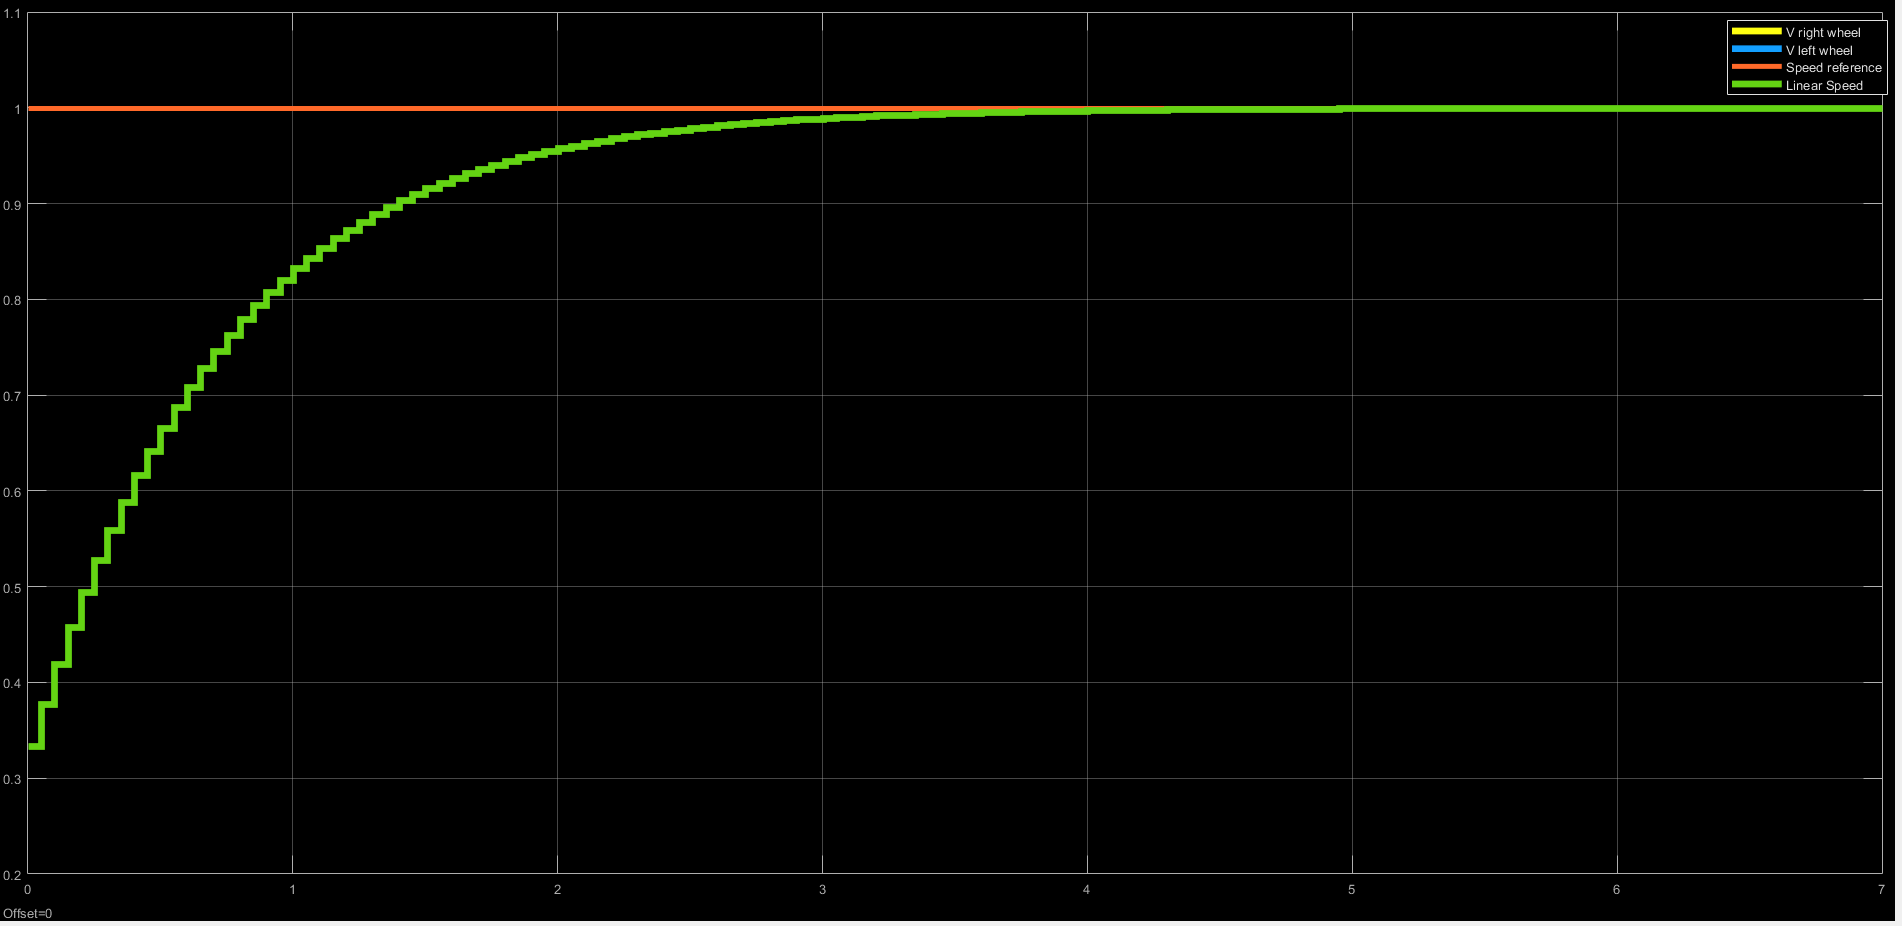
\includegraphics[width=0.8\textwidth]{./img/vel10.png}
\caption {\label{fig:sim1 - vel}Linear speed with reference v=1m/s,$\theta = 0~\si{rad}$}
\end{figure}
 As expected,the figure \ref{fig:sim1 - vel} shows that the car linear velocity reached 1m/s. The angle of tilt is equal to 0 which means the car will be moving in a straight line, and as such, both wheels will are moving at the same speed of the car.\\
\newpage
\begin{figure}[!h]
\centering
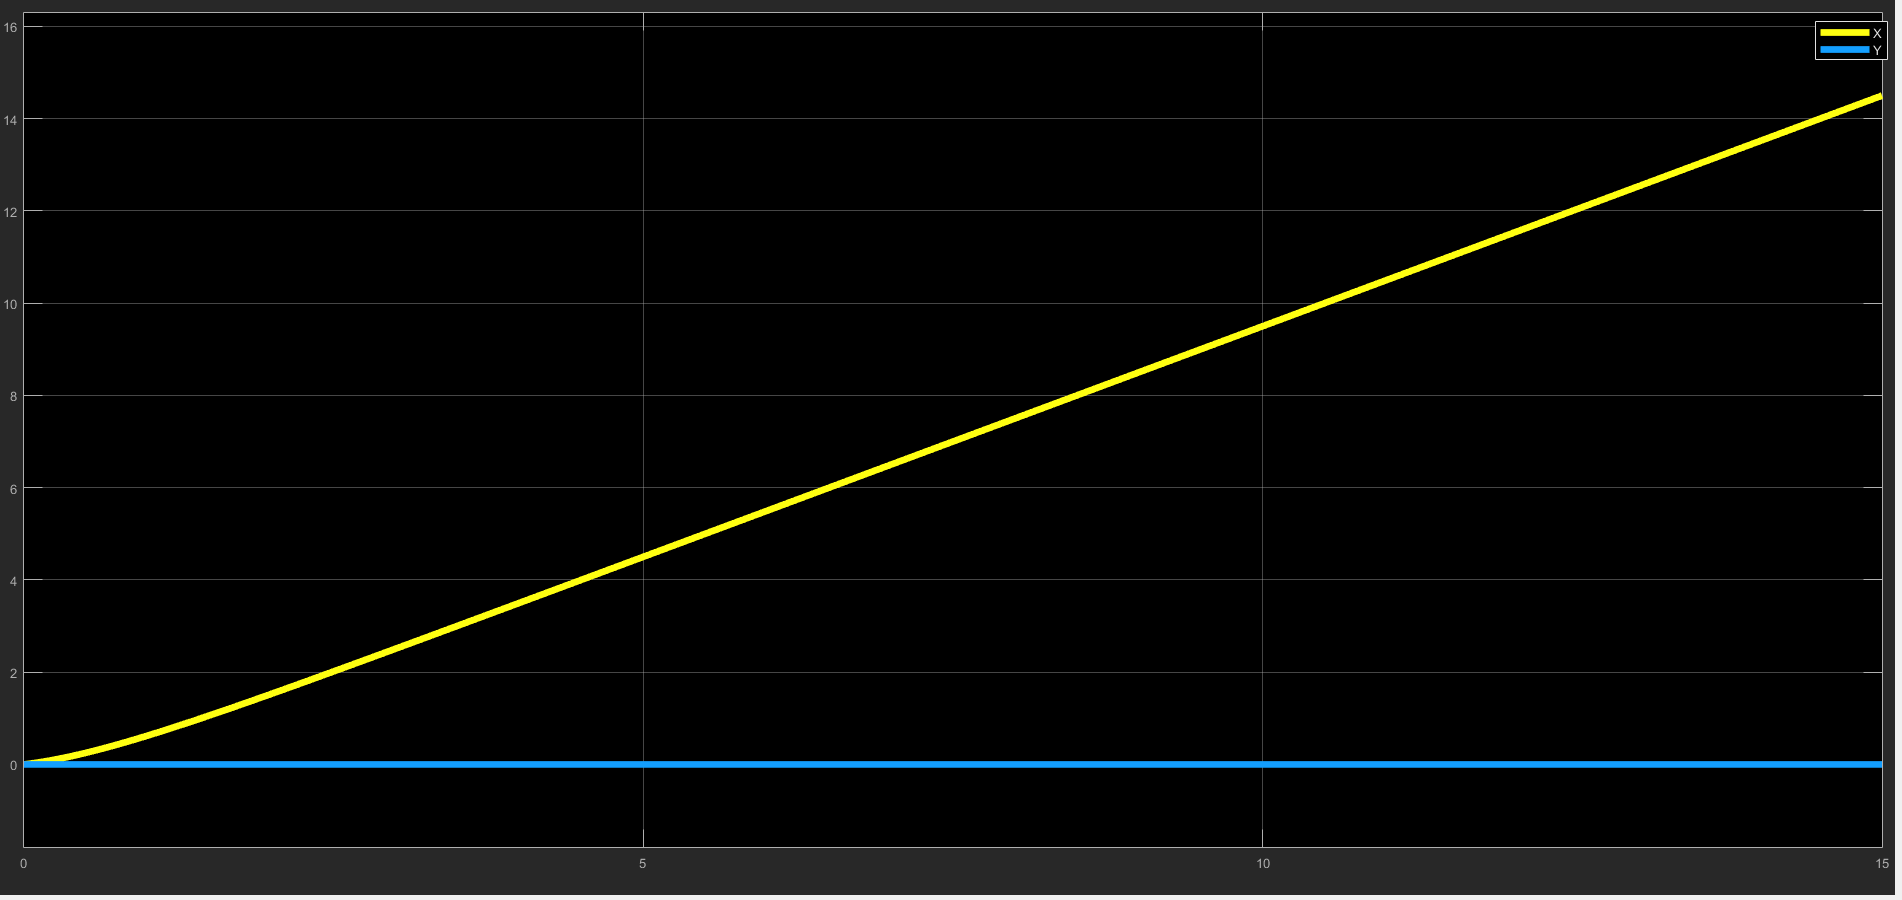
\includegraphics[width=0.8\textwidth]{./img/xy10.png}
\caption {\label{fig:sim1 - pos}Car position(xy) with reference v=1m/s, $\theta = 0~\si{rad}$}
\end{figure}
As the $\theta$ is equal to 0 rad, only 1 coordinate of the car is moving, as the figure \ref{fig:sim1 - pos} demonstrates. The x coordinate is equal to 0 the entire simulation time, and the y coordinate is increasing with a linear scope equal to the linear velocity of the car. This implies that the car is indeed moving in a straight line.\\
Changing the $\theta$ to 0.1 rad to simulate constant tilt of the smart phone to the right, and maintaining the value of the speed reference in 1 m/s :\


\begin{figure}[!h]
\centering
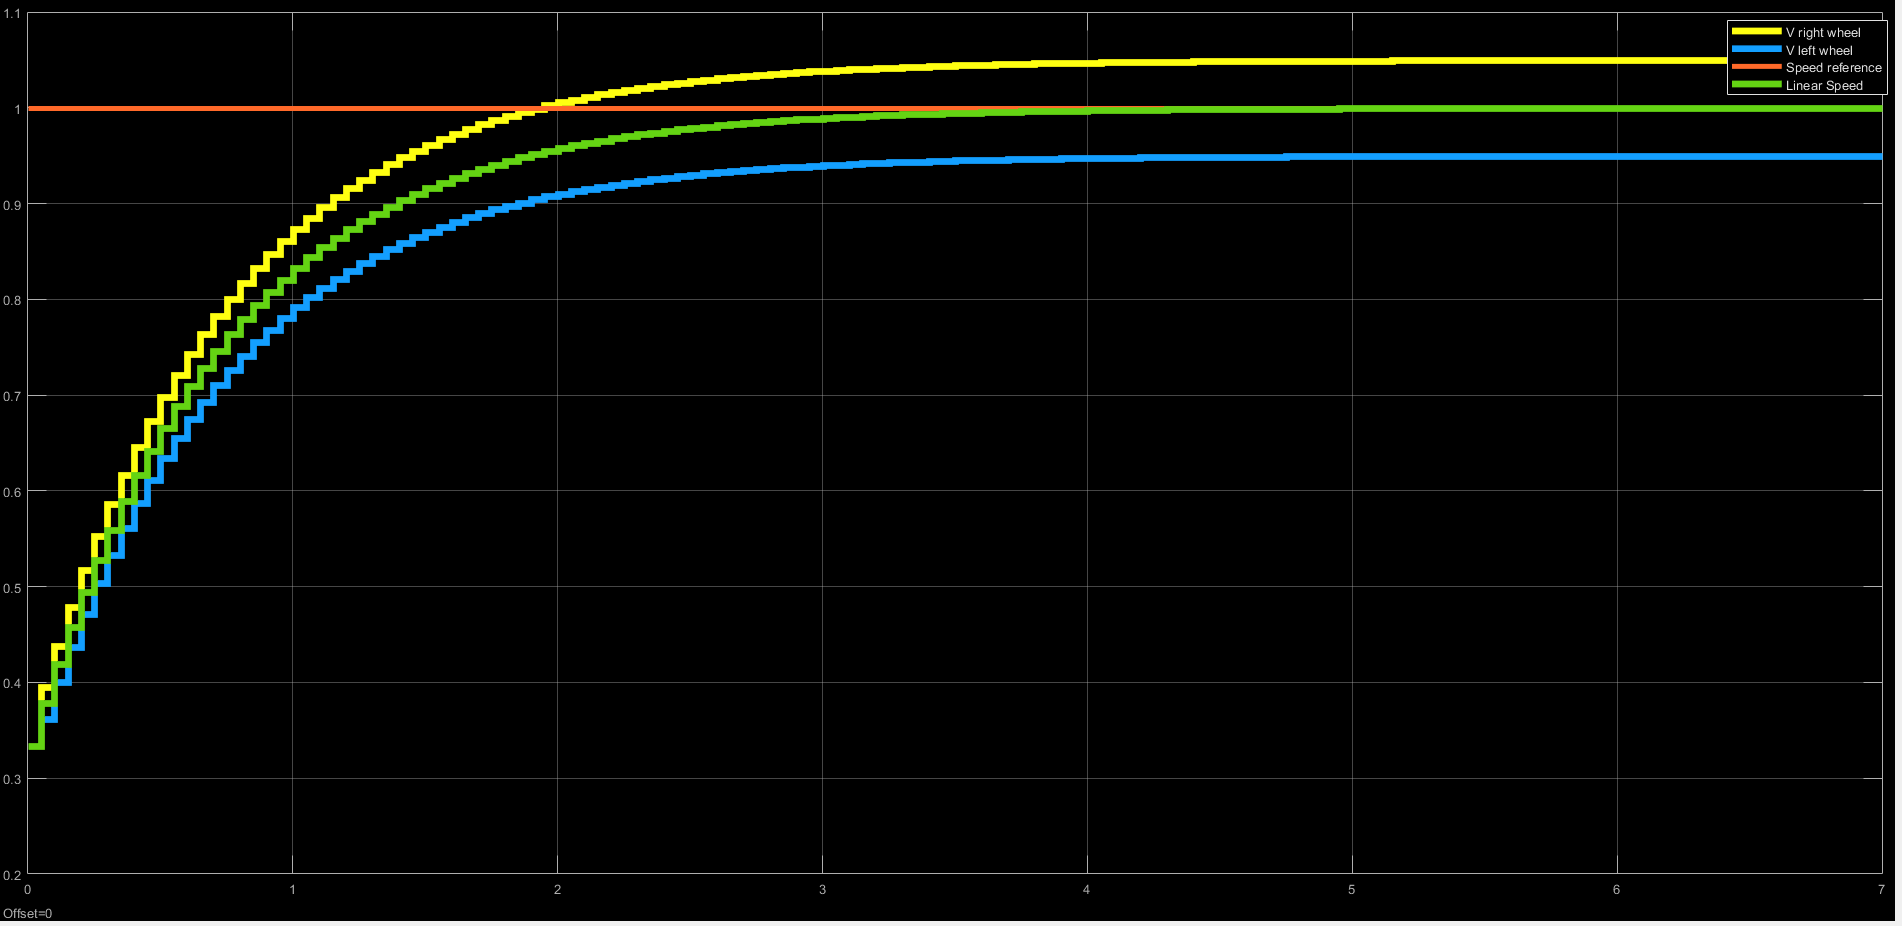
\includegraphics[width=0.8\textwidth]{./img/vel101.png}
\caption {\label{fig:sim2 - vel}Linear speed with reference v=1m/s,$\theta = 0.1~\si{rad}$}
\end{figure}
In the simulation figure \ref{fig:sim2 - vel} it can be observed that having a angle of tilt not equal to 0, causes the left and right wheels to have different velocities, in order to make the car turn. Running more simulations with different values of $\theta$, the outcome shows that the bigger the module of the value of $\theta$, the bigger the difference between the linear velocities of the wheels.\


\begin{figure}[!ht]
\centering
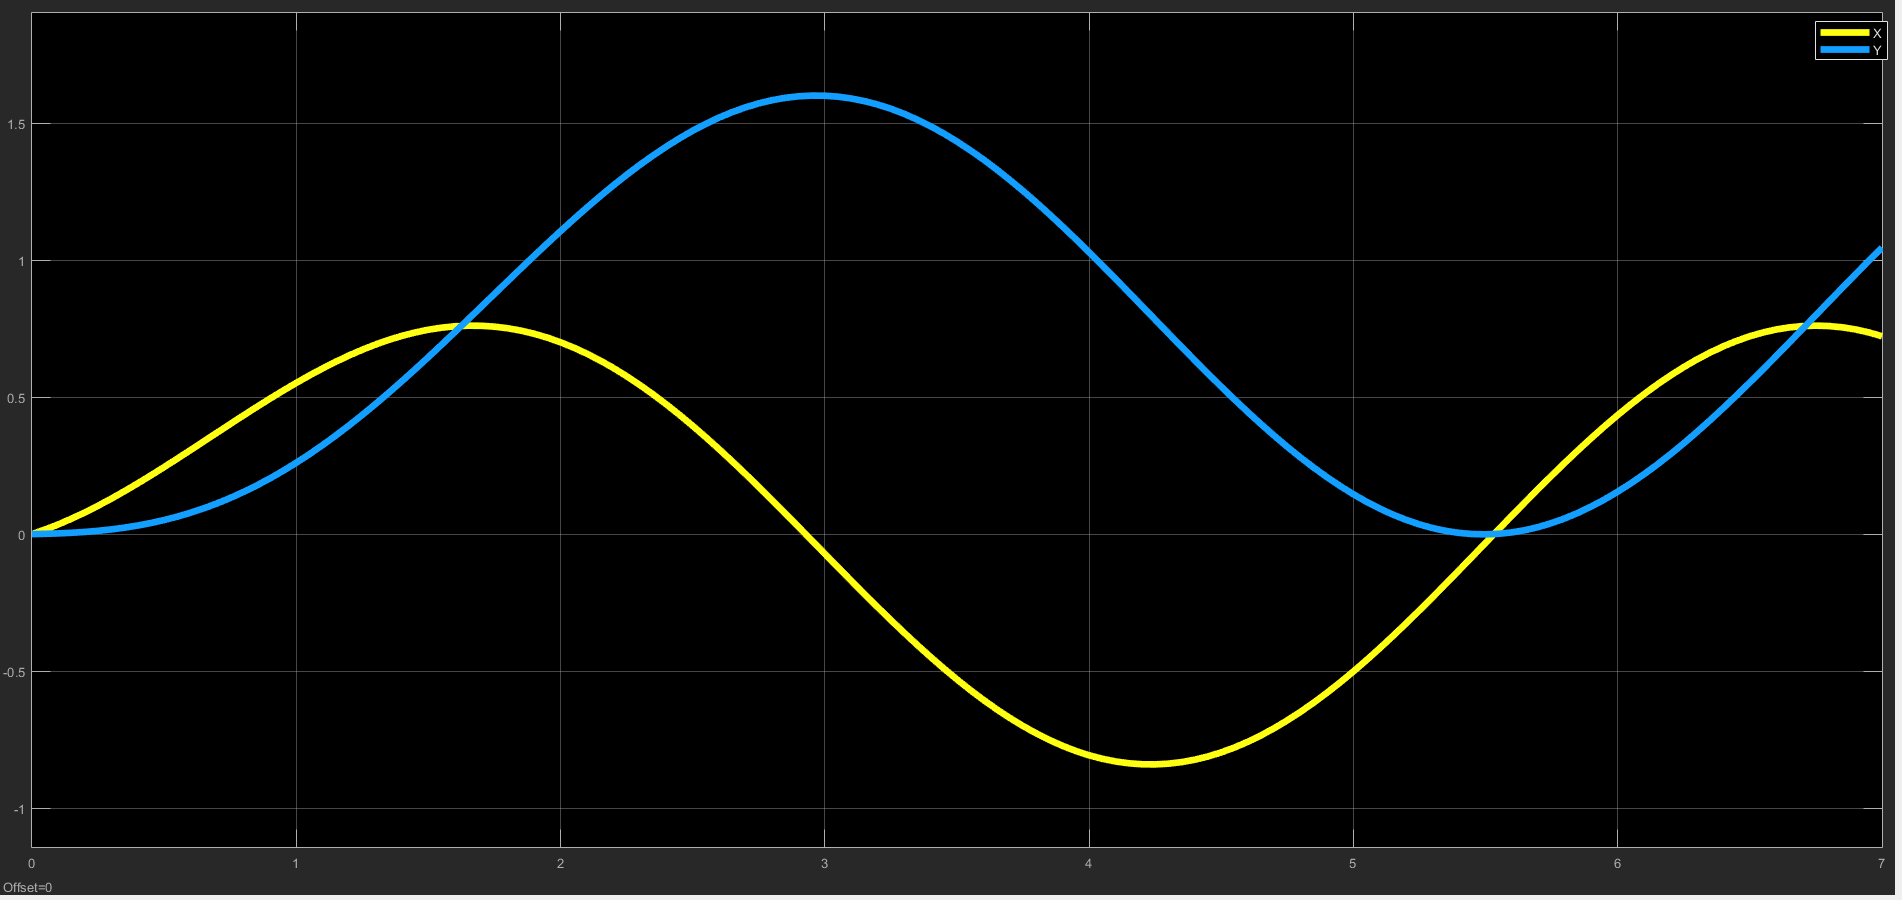
\includegraphics[width=0.8\textwidth]{./img/xy101.png}
\caption {\label{fig:sim2 - pos}Car position(xy) with reference v=1m/s, $\theta = 0.1~\si{rad}$}
\end{figure}
With this figure \ref{fig:sim2 - pos} it is possible to observe that both the
position of x and y of the car change with time. With a constant angle of tilt,
the car will turn constantly in the same direction, eventually making a 360
degrees turn and as the car as small dimensions, it takes a very small time for
it to do so, which is what is observed is this simulation.
%%% Local Variables:
%%% mode: latex
%%% TeX-master: "../../../dissertation"
%%% End:
